\section{时间序列的拓扑表示构建方法}
\subsection{时间序列转化为TDA可处理的表示}
拓扑数据分析(TDA)通过持久同调(Persistent Homology)提取数据的拓扑特征,如连接组件和孔洞,对噪声鲁棒且能揭示复杂数据的内在模式,特别适合处理非线性时间序列。然而,TDA要求数据以点云或复形形式输入,而时间序列为一维数值序列,无法直接应用。因此,需通过时间延迟嵌入(TDE)等方法将时间序列转化为高维点云,以捕捉动态系统的吸引子或拓扑特性。本章将系统介绍时间序列到TDA表示的转化方法,包括时间延迟嵌入(TDE)、值-差分散入等,分析其数学原理、实现步骤和适用场景,为后续特征提取和分类任务奠定基础。本章结构如下图所示:
% 插入图片 路径是figure/第三章.png
\begin{figure}[thbp!]
    \centering
    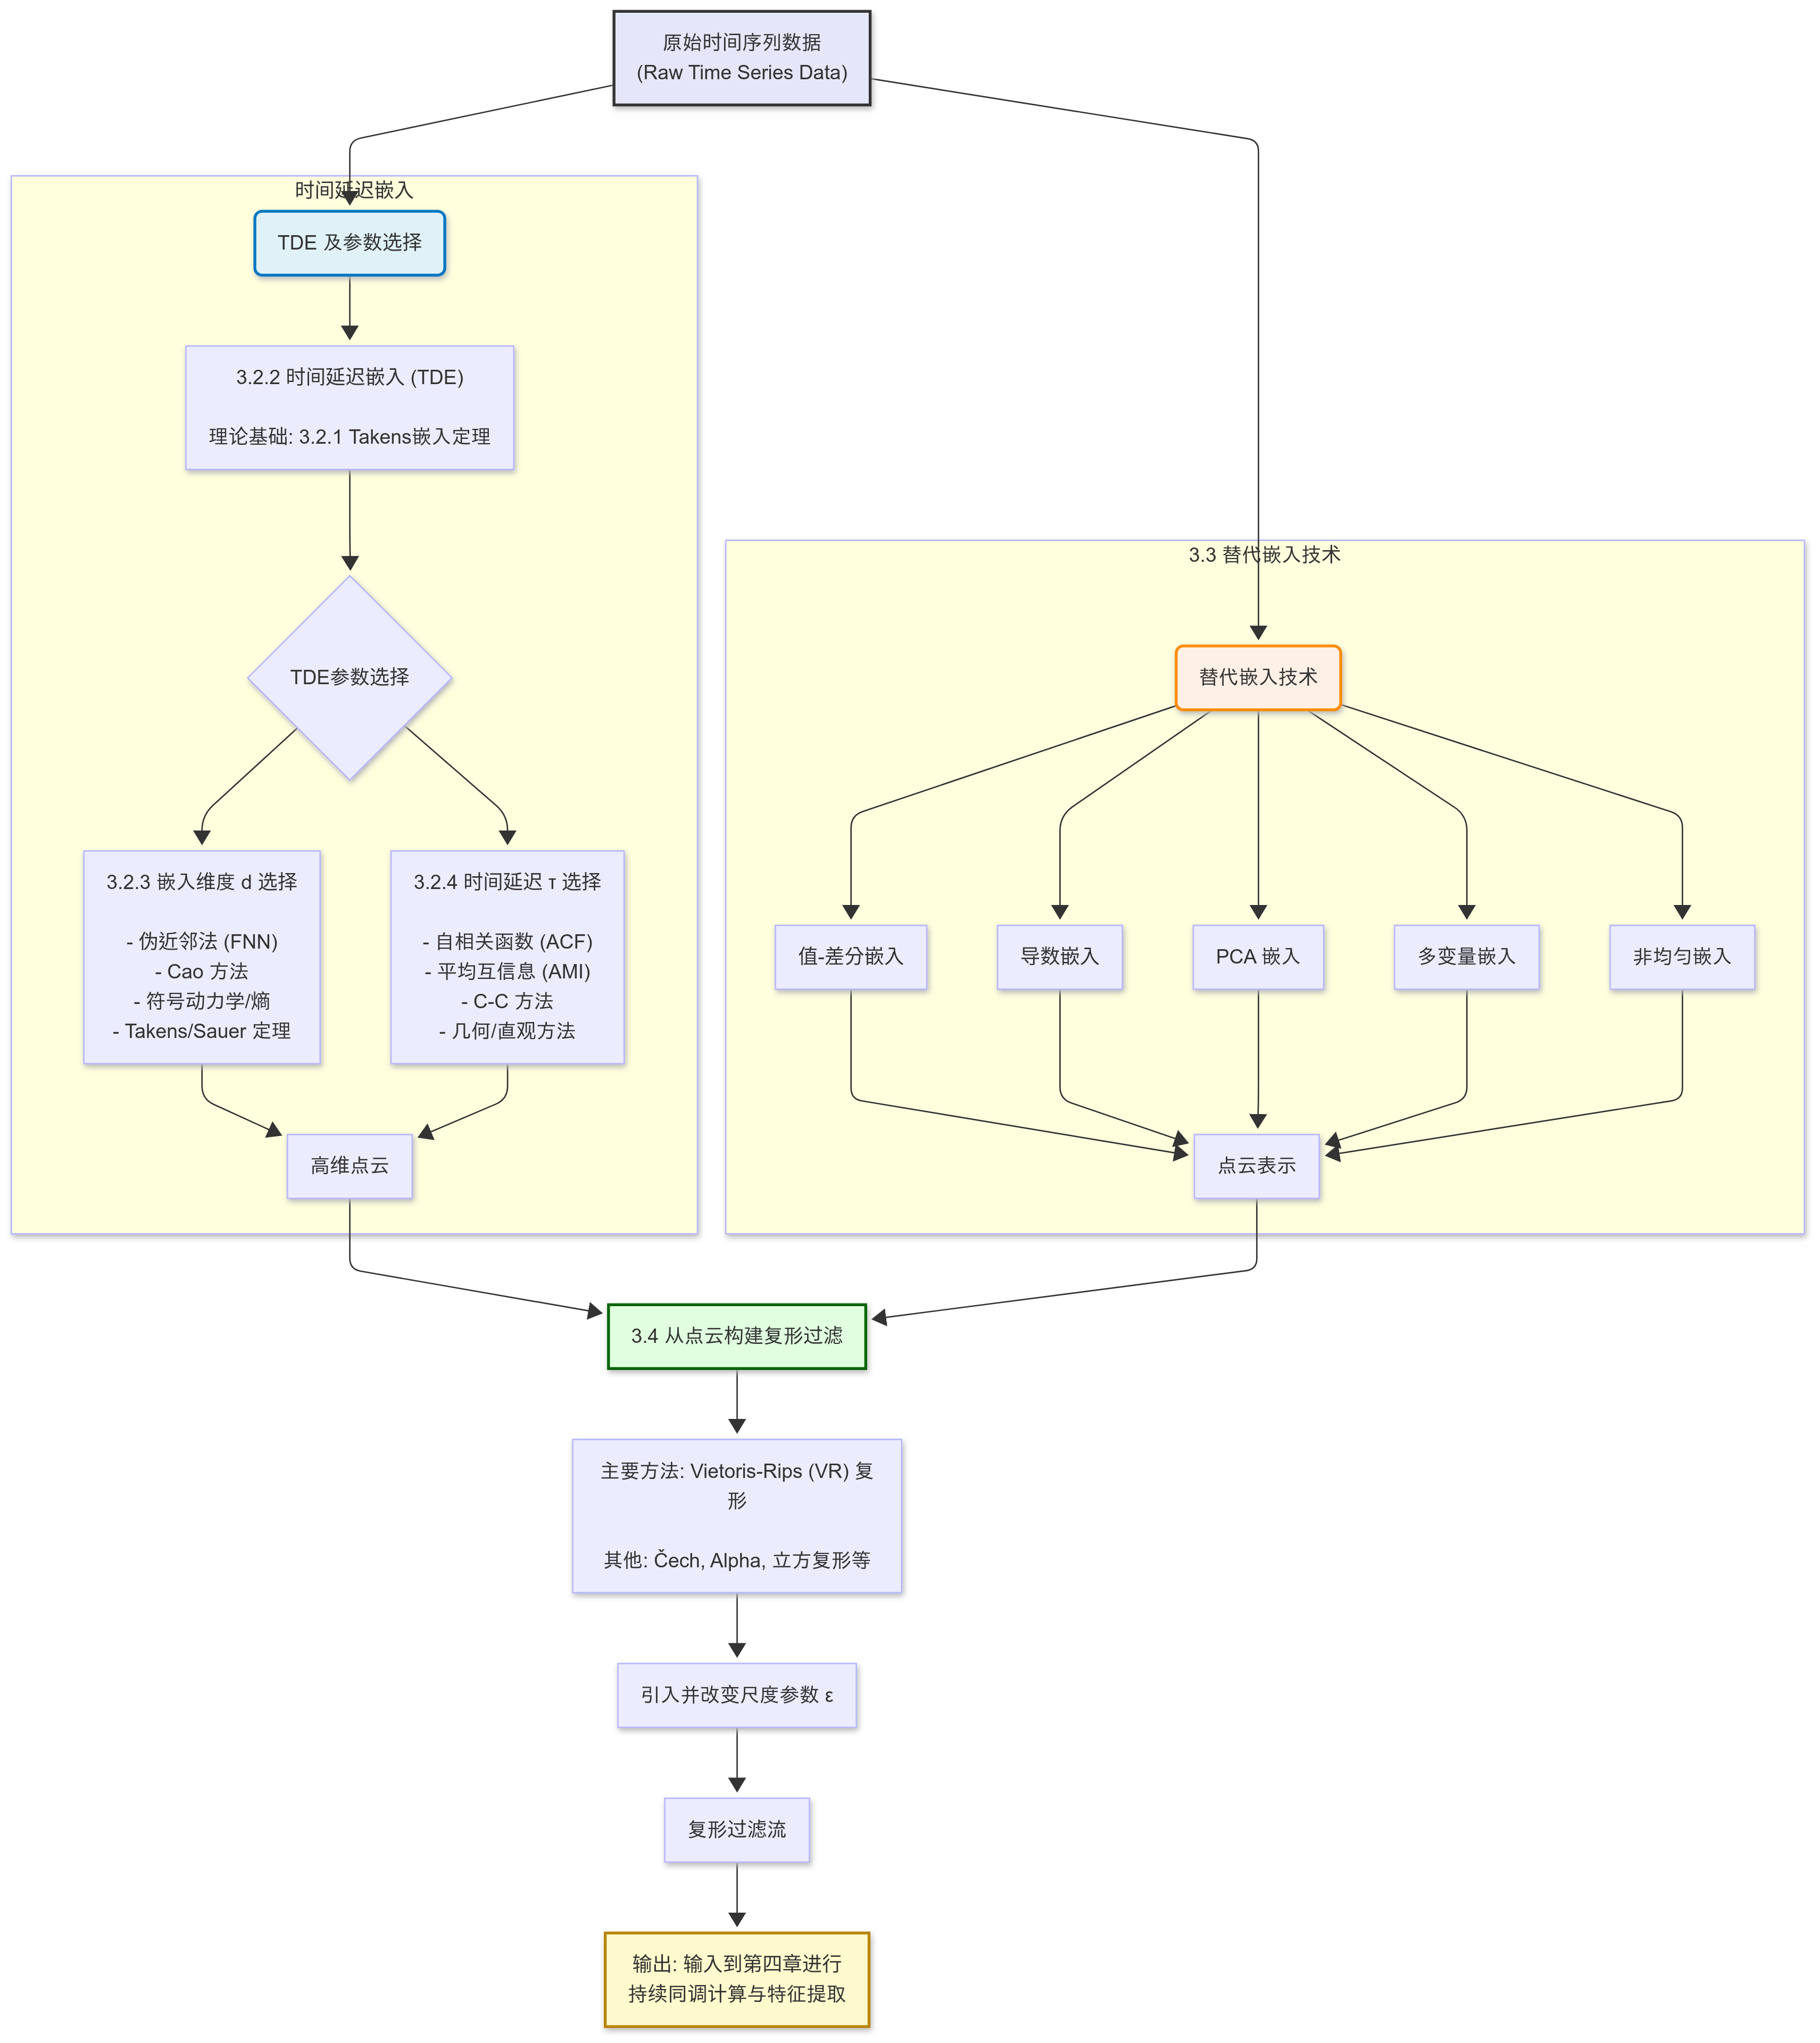
\includegraphics[width=.9\textwidth]{figure/第三章.png}
    \caption{拓扑表示构建流程图}
\end{figure}
 
\subsection{状态空间重构}
我们需要将观测到的时间序列数据重构系统动力学状态空间,并构建其拓扑表示的方法.在许多科学和工程领域,我们面对的是复杂的动态系统,但往往只能观测到系统的一个或少数几个变量随着时间而变化,这种观测导致我们难以理解分析系统完整行为,所以我们需要从有限的,可能带有噪声的观测数据中,推断出驱动系统演化的潜在高维信息.传统的线性时间序列分析方法虽然在某些情况下有效,但往往难以捕捉复杂系统所固有的非线性特征和相互作用.状态空间重构是一个非常的好的解决办法,其基本洗漱是将低维的时间序列数据,通过特定的嵌入技术,转化为一个高维空间中的几何对象,这个重构出的状态空间在理想情况下能保持原始系统动力学的主要拓扑和几何特性.在众多状态空间重构技术中,时间延迟嵌入(TDE)扮演着基石性的角色.
\subsubsection{Takens 嵌入定理}
TAKENs嵌入定理(Takens' Embedding Theorem)\cite{takens2006detecting}是由荷兰数学家Floris Takens在1981年提出的一个重要数学定理,主要应用于动力系统和时间序列分析领域。它提供了一种从单一标量时间序列数据中重构原始动力系统相空间的方法,尤其在研究混沌系统和非线性动力学时具有深远意义。

在介绍定理之前我们先来介绍两个基本概念:
\begin{itemize}
    \item \textbf{相空间(Phase Space)}: 动力系统的状态空间,描述系统所有可能状态的集合。对于一个n维动力系统,相空间是n维的。
    \item \textbf{吸引子(Attractor)}: 动力系统在长时间演化后趋向的状态或轨迹集合。吸引子可以是点、周期轨道或更复杂的结构,如奇异吸引子。
\end{itemize}
TAKENS嵌入定理的核心思想是,通过对时间序列进行适当的嵌入,可以在高维空间中重构出原始动力系统的相空间结构。具体来说,假设我们有一个一维时间序列$x(t)$,它是一个动力系统在时间上的投影。TAKENS定理指出,如果我们选择合适的嵌入维度$d$和时间延迟$\tau$,那么通过以下方式构造的$d$维向量序列可以近似重构原始动力系统的相空间:
\begin{equation}
    \mathbf{x}_i = (x(t_i), x(t_{i+\tau}), x(t_{i+2\tau}), \ldots, x(t_{i+(m-1)\tau}))
\end{equation}
其中,$i$是时间序列的索引,$t_i$是时间点,$d$是嵌入维度,$\tau$是时间延迟。

TAKENS定理的直观解释是:由于确定性动力系统中各个状态变量是相互耦合的,当前观测值及其过去(或未来)的延迟值序列中,蕴含了关于当前未被直接观测到的其他状态变量的信息.
补充: sauer等人将嵌入维度$d$的下限给出为$m\geq 2d+1$,其中$d$是原始系统的维数.这个定理的一个重要结论是,只要嵌入维度足够大,就可以通过重构的相空间来恢复原始系统的动力学行为,包括吸引子结构和混沌特性.



\subsubsection{时间延迟嵌入 (TDE)}
时间延迟嵌入(Time Delay Embedding, TDE) 是一种将一维时间序列数据转化为高维点云的技术,基于 Takens 嵌入定理。TDE 的基本思想是通过引入时间延迟和嵌入维度,将时间序列中的每个观测值与其过去的观测值组合成一个高维向量,从而重构出系统的相空间。这种方法能够捕捉到系统的非线性动力学特征,如周期性、混沌行为等。
TDE 的基本原理是将一维时间序列 \( s(t) \) 通过引入时间延迟 \( \tau \) 和嵌入维度 \( d \),转化为高维向量:
\begin{equation}
\vec{x}(t) = \left[ s(t), s(t - \tau), s(t - 2\tau), \dots, s(t - (d - 1)\tau) \right]
\end{equation}
这些向量构成的集合形成了一个高维点云,即重构的相空间。Takens 定理指出,当嵌入维度 \( d \geq 2m + 1 \)(其中 \( m \) 为原始系统的维数)时,重构的相空间与原始系统的相空间拓扑等价。这种重构使得我们可以从单一观测变量中恢复系统的非线性动力学行为,例如吸引子结构或混沌特性。点云中的每个点代表系统在某时刻的状态,而点云的几何形状则反映了系统的长期演化规律。


\subsubsection{嵌入维度参数\(d\)的选择}
时间延迟嵌入(TDE)中嵌入维度 $d$ 的选择,直接决定了重构状态向量 $\vec{y}(t) = [x(t), \dots, x(t+(m-1)\tau)]$,对能否有效重构系统动力学至关重要。一个充分的 $d$ 值是保证重构空间能真实反映原始吸引子拓扑结构的基础。

若 $d$ 值选取 \textbf{过低},重构空间不足以完全“展开”高维吸引子,会导致原本分离的轨迹因投影而错误地靠近,产生所谓的 “伪近邻” (FNN)。这种拓扑结构的扭曲会严重影响后续基于重构空间的分析。

反之,若 $d$ 值选取 \textbf{过高},则会引入 “维度灾难” 问题。在有限数据下,高维空间的数据点变得稀疏,降低了依赖局部密度估计的分析方法(如关联维计算)的可靠性。同时,高维度也增加了计算负担并可能放大噪声。

因此,目标是找到最小的充分嵌入维度 $m_{min}$,它既能完全展开吸引子(消除FNN),又能避免不必要的高维问题。虽然Takens等理论给出了维度的理论下界(如 $m \ge 2d+1$ 或 $m > 2d_A$),但通常需要根据数据进行估计。

实践中常用数据驱动方法估计 $d$。伪近邻法 (FNN)\cite{rhodes1997false}通过考察随着维度从 $d$ 增加到 $m+1$,近邻点对的距离是否显著增大来判断维度是否充分。当伪近邻比例降至阈值以下时,对应的 $d$ 可视为一个充分估计。Cao方法\cite{cao1997practical} 是对FNN的改进,通过分析统计量 $E1(m)$(邻近点距离的平均相对变化率)随 $d$ 的饱和行为来确定 $d$,并用 $E2(m)$ 辅助判断数据是否具有确定性。

总之,$d$ 的选择是一个需要在保证拓扑嵌入有效性与避免高维问题之间进行权衡的经验过程。通常需要结合使用多种估计方法,并考虑数据特性(长度、噪声)及分析目标。对估计值附近的 $d$ 进行敏感性分析,检验后续结果的稳定性,是验证选择合理性的常用手段。以下是一些常用的方法:
\newpage
% --- End of LaTeX Snippet ---

\begin{table}[h!] % 使用 [h!] 尝试将表格放置在此处
    \centering % 表格居中
    \caption{时间延迟嵌入嵌入维度($d$)选择方法对比(不含优点和缺点)}
    \label{tab:embedding_dimension_methods_no_pros_cons}
    \begin{tabular}{
      >{\raggedright\arraybackslash}m{3cm} % 方法名称 (左对齐,自动换行)
      >{\raggedright\arraybackslash}m{4.5cm} % 核心原理 (左对齐,自动换行)
      >{\raggedright\arraybackslash}m{5cm}  % 原理阐释 (左对齐,自动换行)
      >{\raggedright\arraybackslash}m{4cm}  % 常用判据 (左对齐,自动换行)
    }
    \toprule % 顶部线条
    \textbf{方法名称} & \textbf{核心原理}  & \textbf{原理阐释}  & \textbf{常用判据/解释} \\
    \midrule % 中间线条
    
    伪近邻法 (FNN) \cite{rhodes1997false}& 邻近点在维度增加时的相对距离变化  & 维度不足时,投影导致假邻居;维度足够时,假邻居会散开,真邻居保持靠近  & \%FNN随 $d$ 增加首次降至零或小阈值  \\
    \addlinespace % 增加行间距
    
    Cao方法\cite{cao1997practical} & 近邻点对距离相对变化率的平均值 ($E1(m)$)  & 旨在改进FNN,减少对阈值的依赖;观察变化率何时稳定  & 绘制 $E1(m)$ 曲线,寻找其趋于平稳的 $d$ 值 。$E2(m)$ 用于区分确定性与随机性  \\
    \addlinespace
    
    符号动力学/熵方法 & 符号序列的熵  & 利用熵度量信息量或依赖性随参数的变化;将 $d$ ($p$), $τ$ 与最优时间窗口 $\tau_w$ 关联  & 寻找使熵最大化($\tau^*$)和最小化($\tau_w$)的延迟,通过 $\tau_w=(p-1)\tau^*$ 定 $p$  \\
    \addlinespace
    
    Takens/Sauer 定理 (理论基础) & 保证嵌入的微分同胚性  & 足够高的维度能“展开”吸引子,保持拓扑结构  & 理论要求 $m > 2d$ (Takens) 或 $m > 2d_A$ (Sauer),其中 $d$ 为系统维数,$d_A$ 为吸引子盒维数 \\
    
    \bottomrule % 底部线条
    \end{tabular}
    \par % 确保表格后的文本在新行开始
    \vspace{0.5cm} % 在表格后增加一些垂直空间
    \textit{注意:实际应用中选择嵌入维度 $d$ 通常是一个启发式过程,可能需要结合数据特性和析目标进行权衡 。FNN 和 Cao 方法旨在估计最小且足够的 $d$ 。}
    \end{table}
下面我来介绍一下cao方法在论文中的运用:
曹亮月\cite{cao1997practical}提出的确定标量时间序列最小嵌入维数 $d_{min}$ 的方法,其核心思想是避免传统方法中主观参数的选择。该方法首先定义一个量 $a(i,d)$:
\begin{equation}
a(i,d) = \frac{||y_i(d+1) - y_{n(i,d)}(d+1)||}{||y_i(d) - y_{n(i,d)}(d)||}
\end{equation}
其中 $y_i(d)$ 是 $d$ 维重构相空间中的点,$y_{n(i,d)}(d)$ 是其最近邻。然后计算 $a(i,d)$ 的均值 $E(d)$:
\begin{equation}
E(d) = \frac{1}{N-d\tau}\sum_{i=1}^{N-d\tau} a(i,d)
\end{equation}
并考察其变化率 $E1(d)$:
\begin{equation}
E1(d) = E(d+1)/E(d)
\end{equation}
当 $d$ 大于某个值 $d_0$ 后,$E1(d)$ 趋于饱和,此时 $d_0+1$ 即为最小嵌入维数。为区分确定性与随机信号,还引入了 $E^*(d)$:
\begin{equation}
E^*(d) = \frac{1}{N-d\tau}\sum_{i=1}^{N-d\tau} |x_{i+d\tau} - x_{n(i,d)+d\tau}|
\end{equation}
及其变化率 $E2(d)$:
\begin{equation}
E2(d) = E^*(d+1)/E^*(d)
\end{equation}
对于随机数据,$E2(d)$ 对所有 $d$ 均约等于1。下表总结了论文中部分实验结果:

\begin{table}[h!]
    \centering
    \caption{曹氏方法实验结果选例}
    \begin{tabular}{|l|l|l|l|}
    \hline
    \textbf{系统} & \textbf{数据长度} & \textbf{Cao方法 $d_{min}$} & \textbf{备注/FNN对比} \\
    \hline
    Hénon 吸引子 & 1000 \& 10000 & 2 & 结果对数据长度不敏感 \\
    \hline
    Ikeda 吸引子 & 1000 \& 10000 & 4 & 1000点时FNN结果不稳定 \\
    \hline
    Lorenz 吸引子 & 1000 \& 10000 & 3 & 结果稳定 \\
    \hline
    随机有色噪声 & 1000 \& 10000 & N/A ($E2 \approx 1$) & FNN方法会误判为低维混沌 \\
    \hline
    Mackey-Glass ($\Delta=100$) & 1000 \& 10000 & 17 & FNN方法结果偏小 ($\sim$6)且依赖参数 \\
    \hline
    特定四维映射 & 1000 \& 10000 & 4 & 1000点时FNN无法区分,万点结果也不稳 \\
    \hline
    实验激光数据 & 1000 & 7 & FNN结果在$d=7$后不稳定 \\
    \hline
    \end{tabular}
    \end{table}

    曹亮月通过对Hénon映射、Ikeda映射、Lorenz吸引子、随机有色噪声、高维Mackey-Glass方程、特定四维映射及真实激光数据等多种时间序列的实验验证了其方法的有效性。实验结果表明,该方法不仅能准确确定不同动力系统的最小嵌入维数 $d_{min}$,且对数据长度不敏感;尤为重要的是,它能有效区分确定性混沌与随机信号(如随机有色噪声,此时$E2(d) \approx 1$),并在处理高维系统(如Mackey-Glass)时显著优于传统的虚假最近邻(FNN)方法,后者在这些情况下常给出偏低或不稳定的结果且依赖于参数选择 。这些实验共同证明了曹氏方法在确定嵌入维数方面的鲁棒性、客观性和广泛适用性。

\subsubsection{时间延迟参数$\tau$的选择}


在利用时间延迟嵌入技术重构复杂系统相空间的过程中,除了选择合适的嵌入维度 $d$ 之外,时间延迟参数 $\tau$ 的选取同样是\textbf{至关重要}的一环。它直接决定了构成嵌入向量 $\vec{y}(t) = [x(t), x(t+\tau), \dots, x(t+(m-1)\tau)]$ 各分量之间的时间间隔。一个恰当的 $\tau$ 值是保证重构相空间能够有效“展开”原始动力系统吸引子,并保持其拓扑结构不变性的关键因素之一。

选择一个过小的 $\tau$ 值,会导致嵌入向量的相邻分量之间线性相关性过强,信息冗余度高。此时,$x(t)$ 与 $x(t+\tau)$ 非常接近,它们并未提供足够多的“新”信息来区分邻近的轨迹段。结果是,重构出的吸引子可能仍然是“折叠”或“挤压”在一起的,未能充分展现其在高维空间中的真实几何形态,这无疑会扭曲我们对系统动力学行为的理解。

相反,如果选择一个过大的 $\tau$ 值,虽然可以保证各分量之间的线性无关性甚至统计独立性,但 $x(t)$ 与 $x(t+(m-1)\tau)$ 之间可能已经失去了系统内在的动力学关联。这相当于在时间上跳跃得太远,使得嵌入向量无法捕捉到系统轨迹的连续演化特征和确定性结构,重构出的相空间可能变得杂乱无章,甚至接近随机噪声的表现,同样无法真实反映原始动力学。

因此,$\tau$ 的选择面临着一个\textbf{核心的权衡}:既要足够大以确保嵌入向量的各分量包含足够独立的信息,从而有效展开吸引子;又要足够小以保留系统随时间演化的内在关联性与动力学规律。一个不恰当的 $\tau$ 值将直接影响后续所有基于重构相空间的分析,包括分形维数的计算、Lyapunov 指数的估计、系统的预测精度以及噪声抑制的效果等。鉴于其对整个相空间重构质量和后续分析有效性的\textbf{决定性影响},如何合理地选择时间延迟 $\tau$ 成为了时间序列非线性分析中的一个基本且关键的问题。下面将展示几种常用的 $\tau$ 值选择策略及其背后的原理。


\begin{table}[h!] % 使用 [h!] 尝试将表格放置在此处
    \centering % 表格居中
    \caption{时间延迟嵌入时间延迟 ($\tau$) 选择方法对比} % 表格标题
    \label{tab:time_delay_tau_methods_compare} % 用于交叉引用的标签
    \begin{tabular}{
      >{\raggedright\arraybackslash}m{3cm}    % 方法名称 (左对齐,自动换行,宽度 3cm)
      >{\raggedright\arraybackslash}m{4.5cm}  % 核心原理 (左对齐,自动换行,宽度 4.5cm)
      >{\raggedright\arraybackslash}m{5cm}   % 原理阐释 (左对齐,自动换行,宽度 5cm)
      >{\raggedright\arraybackslash}m{4cm}    % 常用判据 (左对齐,自动换行,宽度 4cm)
      % 注意:总宽度 3+4.5+5+4 = 16.5cm,加上列间距可能超出典型 A4 页边距下的文本宽度
      % 如遇表格超出页面,请尝试减小 m{} 列的宽度值
    }
    \toprule % 顶部线条 (来自 booktabs)
    \textbf{方法名称} & \textbf{核心原理} (分析的度量) & \textbf{原理阐释} (为何有效) & \textbf{常用判据/解释} \\
    \midrule % 中间线条 (来自 booktabs)
    
    自相关函数 (ACF) & 时间序列与其滞后版本间的线性相关性  & 寻找 $x(t)$ 与 $x(t+\tau)$ 线性无关的最小延迟  & $\tau$ 取 ACF 首次降至零  或首次降至 $1/e \approx 0.37$  的值 \\
    \addlinespace % 增加行间距 (来自 booktabs)
    
    平均互信息 (AMI)\cite{wallot2018calculation} & $x(t)$ 与 $x(t+\tau)$ 之间的统计依赖性 (信息论度量)  & 寻找 $x(t)$ 与 $x(t+\tau)$ 共享信息量最少的延迟,以捕捉非线性结构  & $\tau$ 取 AMI 函数 $I(\tau)$ 的第一个局部最小值  \\
    \addlinespace
    
    C-C 方法 (基于关联积分) & 分析关联积分在不同 $\tau, m$ 下随邻域半径 $r$ 的变化 [...] & 通过检验不同时间窗内数据的统计独立性与几何展开程度寻找最优参数  & 寻找特定统计量(如 $\Delta \bar{S}_2(t)$ 或 $\sigma_{cor}(t)$)首次穿零或达极小值对应的 $t$ (即 $\tau$)  \\
    \addlinespace
    
    几何/直观方法 & 观察时间序列图或相图的特征时间尺度  & 基于对系统动力学行为的先验知识或直观观察估计 & $\tau$ 常取为主要周期或特征时间的某个分数(如 1/4 到 1/10)\\
    
    \bottomrule % 底部线条 (来自 booktabs)
    \end{tabular}
    \par % 确保表格后的文本在新行开始
    \vspace{0.5cm} % 在表格后增加一些垂直空间
    \textit{注意:选择 $\tau$ 与选择 $d$ 密切相关。实际应用中 $\tau$ 的选择常带有启发性,需测试不同值的影响 [...]。AMI 通常被认为是较优选择 [...]。[...]处请替换为实际引用。}
    \end{table}

\textbf{相关实验}: Wallot 和 Mønster(2018)\cite{wallot2018calculation} 该实验选择时间嵌入参数时,首先使用平均互信息(AMI)确定延迟参数 $\tau$。对于一维时间序列 $x(t)$,AMI 的计算公式为
$$I(x(t),x(t+\tau))=\sum_{i,j}p_{ij}(\tau)\log\left(\frac{p_{ij}(\tau)}{p_{i}p_{j}}\right)$$
其中 $p_i$ 是数据点在直方图第 $i$ 个bin的概率,$p_{ij}(\tau)$ 是 $x(t)$ 在 bin $i$ 且 $x(t+\tau)$ 在 bin $j$ 的联合概率。对于 $d$ 维时间序列,采用各维度 AMI 的平均值。选择 $\tau$ 的依据是 $I(\tau)$ 的第一个局部最小值或其值首次低于某个阈值(例如 $1/e$)。确定 $\tau$ 后,使用虚假最近邻(FNN)方法选择嵌入维度 $D_{emb}$(这里 $D_{emb}$ 指的是对原始 $d$ 维时间序列进行嵌入的次数)。对于 $d$ 维时间序列 $x_j(t)$,在由 $D_{emb}$ 次嵌入(每次嵌入增加 $d$ 个维度)构成的相空间中,点 $y(t)$ 与其第 $r$ 个最近邻 $y^{(r)}(t)$ 的欧氏距离平方为
$$R_{D_{emb},d}^{2}(t,r)=\sum_{j=1}^{d}\sum_{k=0}^{D_{emb}-1}[x_{j}(t+k\tau)-x_{j}^{(r)}(t+k\tau)]^{2}$$
当增加一次嵌入到 $D_{emb}+1$ 时,新的距离平方为
$$R_{(D_{emb}+1),d}^{2}(t,r)=R_{D_{emb},d}^{2}(t,r)+\sum_{j=1}^{d}[x_{j}(t+D_{emb}\tau)-x_{j}^{(r)}(t+D_{emb}\tau)]^{2}$$
如果从 $D_{emb} \times d$ 维到 $(D_{emb}+1) \times d$ 维时,邻居间的距离发生显著变化(依据阈值 $R_{tol}$ 和 $A_{tol}$ 判断),则该邻居为虚假最近邻。选择使FNN百分比降至接近零的最小 $D_{emb}$ 值,最终的嵌入相空间维度为 $d \times D_{emb}$。

% 加粗总结
\textbf{总结}: 
嵌入维度 $d$ 的选择旨在确保重构空间具有足够的维度,以完全“展开”动力系统的吸引子,避免因维度不足导致的轨迹交叉和结构误判(即伪近邻现象)。我们探讨了多种估计最小充分嵌入维度的方法,包括基于几何直观的伪近邻法 (FNN) 及其改进(如 Cao 方法),以及基于系统理论的 Takens/Sauer 定理等。FNN 及其变种通过考察邻近点在维度增加时的相对距离变化来寻找合适的 $d$,而理论定理则提供了嵌入有效性的数学保证,但其给出的往往是维度的上限而非最优实用值。

时间延迟 $\tau$ 的选择则关注于如何设置嵌入向量中各分量之间的时间间隔,以在保证分量间足够统计独立性(从而有效利用 $d$ 维空间)与保留系统时间演化内在关联性之间取得平衡。$\tau$ 过小导致信息冗余,$\tau$ 过大则可能丢失动力学信息。常用的 $\tau$ 选择方法包括分析时间序列自相关性(如自相关函数 ACF 法,主要关注线性相关)和信息论依赖性(如平均互信息 AMI 法,能更好地处理非线性相关),以及一些试图结合几何特性或同时考虑 $d$ 和 $\tau$ 的方法(如 C-C 方法)。其中,AMI 方法因其对非线性动力学的适应性而被广泛推荐。

值得强调的是,$d$ 和 $\tau$ 的选择并非完全独立的过程。它们共同定义了重构所利用的时间跨度,即所谓的“时间窗口” $\tau_w = (m-1)\tau$ [...]。某些方法(如 C-C 方法)正是着眼于这个时间窗口的优化。更重要的是,实际应用中参数的选择往往带有启发性,不存在一个适用于所有类型时间序列(如长/短、含噪/纯净、周期/混沌)的通用“万能”方法。

因此,在实践中,研究者通常不会仅仅依赖单一方法的建议值,而是倾向于尝试应用多种不同的方法(例如结合几何类、信息论类等手段)来估计 $d$ 和 $\tau$,并对结果进行相互比较和验证。同时,必须充分考虑所分析时间序列的具体特性,例如其采样频率、噪声水平以及内在的特征时间尺度等,这些因素都可能影响不同选择方法的表现和适用性。进行参数敏感性分析也极为关键:考察在一个根据初步方法确定的合理 $d$ 和 $\tau$ 参数值邻域内,后续计算得到的动力学不变量(如关联维、Lyapunov指数)或模型的预测误差是否保持稳定,是验证参数选择鲁棒性的重要手段。最终的选择决策,应当是在综合考量多种方法建议、数据自身特点、参数敏感性测试结果以及具体科学研究目标的基础上作出的。

总而言之,只有通过这样细致、多角度的比较、选择和验证过程,才能更有信心地确保所构建的重构相空间是原始动力系统的一个有效且可靠的拓扑等价表示,从而为后续深入的非线性动力学分析和应用奠定坚实的基础。


% 注意:在你的论文中,你可能需要为这些方法添加参考文献,
% 例如引用 Fraser & Swinney (1986) 关于互信息法的论文,
% 或其他关于吸引子重构和参数选择的综述性文献或教科书。

\subsection{替代嵌入技术}
基于嵌入理论的非线性动力系统分析已广泛应用于时间序列的建模、预测、信号检测与分类。其核心思想是通过嵌入过程从单变量时间序列重构高维状态空间,以揭示系统潜在的动力学特性。Takens嵌入定理为标准的时间延迟嵌入(Time-Delay Embedding, TDE)提供了坚实的理论基础,该方法通过使用信号的延迟副本构建状态向量。

然而,标准的TDE方法在处理真实世界的复杂数据时面临显著挑战。Takens定理的理想化假设(如无限长、无噪声数据)往往难以满足,使得TDE的效果高度依赖于嵌入维数 m 和时间延迟 τ 的精确选择——而这通常缺乏统一标准,且对结果影响巨大。此外,单一的均匀延迟 τ 可能无法有效捕捉具有多个内在时间尺度的复杂系统动力学。

正是这些局限性,尤其是标准TDE在参数选择上的困难以及对多尺度动态捕捉能力的不足,极大地激发了研究者们探索和发展替代性嵌入技术的热情。 这些替代方法旨在从不同角度克服TDE的缺点,例如通过引入导数信息来补充状态描述,利用主成分分析(PCA)优化嵌入维度和方向,采用多变量嵌入整合来自多个传感器或来源的信息,或设计非均匀嵌入以更好地适应变化的或多重的时间尺度。这些技术共同构成了一个更加丰富的嵌入方法工具箱,为从观测数据重构和理解复杂系统动力学提供了更多样化且可能更鲁棒的途径。接下来,我们将介绍其中几种重要的替代嵌入方法。
\subsubsection{值-差分嵌入}
一种直观的替代思路体现在严银凯等人(2024)针对时间序列分类任务所采用的方法中 [23]。他们并未采用高维的TDE,而是选择将原始的单变量时间序列 $\{a_t\}$ 直接映射到一个二维的点云空间。具体地,该方法构建的二维点集 $\{q_t\}$ 中,每一个点 $q_t$ 的坐标由该时刻的观测值 $a_t$ 以及它与下一时刻观测值的一阶差分 $a_{t+1}-a_t$ 构成,即 $q_t = (a_t, a_{t+1}-a_t)$。根据作者的阐述 [20],这种特定的二维构造旨在使生成的点云能够同时反映时间序列的当前状态(由值 $a_t$ 体现)和其短期的变化趋势(由差分 $a_{t+1}-a_t$ 近似),从而捕捉所谓的“周期上和周期内的特征”。

相较于需要仔细调参的标准TDE,这种固定的二维嵌入方式显著简化了嵌入过程,避免了复杂的参数搜索。它为后续应用拓扑数据分析(如持续同调)提供了一种直接的、蕴含了原始值与变化率信息的低维输入表示。尽管这种特定的低维嵌入可能不像满足Takens定理条件的高维TDE那样,能够保证在拓扑意义下完全重构原始动力系统的吸引子,但它代表了在特定研究背景下,为了处理特定问题(如简化流程、突出变化信息)而对嵌入策略进行的适应性构造与尝试。这类方法与其他替代嵌入技术,如导数嵌入、主成分分析嵌入等,共同丰富了从时间序列数据中提取动力学或结构特征的工具箱。

\subsubsection{导数嵌入}
作为时间延迟嵌入(Time-Delay Embedding, TDE)的一种替代性状态空间重构技术,导数嵌入(Derivative Embedding)利用信号的(近似)连续导数来构建嵌入向量。例如,一个包含位置、速度和加速度信息的三维导数嵌入向量可以表示为 $(x(t), \frac{dx}{dt}, \frac{d^2x}{dt^2})$。其核心思想在于,动力系统的状态不仅取决于其当前位置 $x(t)$,也与其变化率(如速度 $\frac{dx}{dt}$、加速度 $\frac{d^2x}{dt^2}$ 等)密切相关。通过将这些导数信息纳入嵌入向量,可以在重构的状态空间中直接捕捉系统的动态变化特性。从理论视角看,导数嵌入可被视为一种基于系统底层微分方程表示来重构其相空间的方法。若一个物理系统能由一组微分方程精确描述,则系统的状态变量及其各阶导数构成了描述该系统演化的自然坐标系。因此,当研究者认为所观测时间序列源自一个由微分方程控制的潜在系统时,导数嵌入提供了一种直观且可能更自然的动力学展开方式,它将分析的焦点从系统的“状态”(由延迟值表示)转移到了系统的“变化”(由导数值表示),为理解那些变化率本身包含关键信息的系统动力学提供了重要的补充视角。

为适应不同的应用需求,导数嵌入的基本概念已被进一步扩展并常与其他技术结合,催生出功能更强大的变体。其中一个重要的变体是导数延迟嵌入(Derivative Delay Embedding, DDE),它被特别设计用于增量式地将时间序列数据转换到嵌入空间,尤其适用于在线流式数据的处理场景。DDE的一个关键优势在于其能够在不依赖于固定窗口长度或数据良好对齐假设的情况下,有效保留数据的内在递归模式,同时保持较高的计算效率,使其非常适合实时捕捉时变特性并进行在线建模与分类任务。另一个值得注意的框架是延迟微分分析(Delay Differential Analysis, DDA),它通常结合了导数信息与非均匀的时间延迟信息,形成所谓的“函数嵌入”(functional embeddings)。通过整合来自不同时间尺度的延迟值和导数值,DDA旨在更全面地刻画复杂系统的动力学特征,能够应用于更广泛的问题,包括处理长度较短或含有缺失值的稀疏时间序列数据。这些变体的出现,例如常与非参数马尔可夫地理模型(MGM)结合构成DDE-MGM方案,反映了导数嵌入的实用价值往往在与其他技术集成时得到显著放大,从而形成更全面的分析框架。

导数嵌入及其变体展现出一系列潜在优势。在计算效率方面,某些方法(如DDE)相较于计算密集型方法(例如动态时间规整DTW)通常具有较低的计算复杂度。特别地,DDE具备良好的在线处理能力,能够处理流式时间序列而无需复杂的预处理(如分割、对齐),适用于需要实时捕捉时变特性并进行建模与分类的应用。此外,这类方法通常对输入数据的假设较少,例如不要求数据具有固定长度或严格对齐,增强了其在多样化现实场景中的适用性。进一步地,DDA等结合多种信息的方法据称对噪声具有一定的鲁棒性,并且能够有效处理短或稀疏的时间序列数据。在分析层面,DDA框架下的导数嵌入特性甚至支持在时域内进行谱分析,例如使用非线性相关函数来检测信号中的频率成分、频率耦合、相位耦合以及进行双谱分析等。从更广泛的系统控制视角看,与导数概念相关的思想(如PID控制器中的微分项)亦有助于预测系统行为,改善系统的稳定性和响应速度,并抑制超调。然而,导数嵌入方法也面临一些固有的局限性。理论与实践之间常常存在差距:尽管理论上可以用导数重构简单低维动力系统的相空间,但对于高维、复杂且通常含有噪声的真实世界系统,进行精确的全局建模往往是不可行的。同时,某些基于导数的方法可能依赖于实践中不完全满足的较强理论假设,有时需要引入正则化等手段来缓解由此产生的不精确性。此外,其适用性也可能受具体应用场景的限制,例如,在针对大型语言模型的特定对抗攻击研究中,若威胁模型关注的是离散的符号(token)层面的扰动而非连续嵌入空间的细微变化,那么基于嵌入空间导数的方法的有效性可能会受到质疑。

尽管存在这些局限性,导数嵌入及其相关概念已在多个领域得到应用。在流式数据分析方面,DDE-MGM方案已被成功用于时间序列的在线建模与分类,据报道在保持高效率的同时取得了先进的性能。生物医学信号处理是另一个重要的应用领域,例如DDA已被用于区分心电图(EKG)数据反映的不同心脏状况,以及区分帕金森病患者与健康对照组的脑电图(EEG)数据。更一般地,导数嵌入可服务于时间序列的信号检测与分类任务。如前所述,DDA等方法还可用于时域内的谱分析,包括频率分析、耦合检测和双谱估计。在金融领域,虽然不直接称为导数嵌入,但相关的随机微分方程(SDEs)是建模资产价格等随机过程的核心工具,对于金融衍生品定价至关重要,其理论基础与导数概念紧密相连。此外,在变化检测领域,许多时间序列变化检测算法是遥感(如利用Landsat时间序列监测地表覆盖变化)和生物监测等应用中的关键组成部分,这些算法有时也隐式或显式地利用了序列的变化率信息。
 
\subsubsection{主成分分析嵌入}
主成分分析(Principal Component Analysis, PCA)是一种经典的线性降维技术,其核心思想是通过正交线性变换将原始高维数据投影到一个新的低维坐标系中,旨在降维的同时尽可能多地保留由方差衡量的原始数据信息。这个新坐标系的轴被称为主成分(Principal Components, PCs),它们相互正交且按照其捕捉到的原始数据方差大小进行排序:第一主成分(PC1)对应数据方差最大的方向,第二主成分(PC2)是在与PC1正交的子空间中方差次大的方向,以此类推。本质上,PCA是在寻找数据变异性最大的方向。

PCA的计算过程通常涉及几个关键步骤。首先,对原始数据的各个特征进行标准化处理,使其具有零均值和单位方差,以消除不同特征尺度差异可能带来的影响。其次,计算标准化后数据特征之间的协方差矩阵,该矩阵反映了特征间的线性相关性。接着,对协方差矩阵进行特征值分解,求解特征向量方程 $AX=\lambda X$(其中 $A$ 是协方差矩阵,$X$ 是特征向量,$\lambda$ 是对应的特征值)。特征向量指明了主成分的方向,而特征值的大小则量化了该主成分所解释的方差。通过将特征值从大到小排序,选择前 $k$ 个最大特征值对应的特征向量,便构成了最优的 $k$ 维投影子空间。最后,将原始标准化数据投影到这个由选定 $k$ 个特征向量张成的子空间上,即可得到降维后的数据表示。

这种将高维数据映射到由主要主成分构成的低维空间的过程,其本身就是一种数据嵌入(Embedding)的方法。这个低维表示试图在更紧凑的空间中保留原始数据的核心结构(以方差最大化为目标)。作为一种无监督的降维技术,PCA在机器学习流程中扮演着重要角色,常被用作预处理步骤,特别是在处理具有极高维度特征的数据时(例如文本分析中的词袋模型、图像数据或基因表达数据)。通过PCA降低维度,可以简化数据表示,减少计算负担,去除部分噪声,并可能提高后续机器学习算法(如分类器、聚类算法)的训练效率和性能。此外,PCA也是探索性数据分析的有力工具,通过将数据投影到二维或三维空间进行可视化,有助于直观理解数据的内在结构、聚类趋势和分布特征。例如,在多变量时间序列(MTS)分析中,可以对表示为矩阵的MTS数据应用PCA,并利用其主成分和特征值来定义MTS之间的相似性度量。

作为一种基础且广泛应用的嵌入与降维技术,PCA具有显著的优点。其计算相对高效,并且作为一种确定性算法,对于给定的数据集每次运行结果都相同。PCA擅长保留数据的全局结构和最大化方差,并且由于其线性变换的本质,其过程和结果相对透明,易于理解和解释(主成分可视为原始特征的线性组合)。同时,PCA也可有效用于数据压缩和降噪。然而,PCA也存在一些固有的局限性。最主要的是其线性假设,使得它可能无法有效捕捉数据中复杂的非线性模式和流形结构。其次,PCA以最大化方差为目标,但这并不总能保证保留对特定下游任务(如分类)最重要的判别信息,例如可能无法很好地区分本身方差不大但类别边界清晰的簇,也可能不如某些方法(如LLE, t-SNE)那样能有效保持数据的局部邻域结构。此外,PCA对原始特征的尺度非常敏感,因此通常需要进行数据标准化预处理。主成分必须相互正交的约束在某些情况下也可能是一种限制。同时,PCA对数据中的离群点也比较敏感。在某些特定领域(如遗传学中表示复杂的混合血统结构),PCA可能不如某些非线性方法或专门设计的模型有效,尽管后者可能面临解释性更差的问题。

尽管存在这些限制,PCA的应用场景依然非常广泛。它被用于数据可视化(降至2D或3D)、加速机器学习模型训练、作为特征提取手段、分析遗传学中的群体结构、在化学与毒理学中处理高维分子指纹数据、预处理自然语言处理中的高维文本表示(如one-hot编码)或融合多领域词嵌入、分析金融领域的新闻嵌入、定义多变量时间序列的相似性度量,以及在研发与专利分析中可视化大型文档集以识别主题簇等。

将PCA与流行的非线性降维或嵌入技术,如变分自编码器(Variational Autoencoder, VAE)、均匀流形逼近与投影(Uniform Manifold Approximation and Projection, UMAP)以及t-分布随机邻域嵌入(t-Distributed Stochastic Neighbor Embedding, t-SNE)进行比较,可以更清晰地理解它们的特性。值得一提的是,具有平方误差损失的线性自编码器在数学上等价于PCA,这为PCA在更广泛的表示学习框架中定位提供了理论联系。VAE是一种基于深度学习的生成模型,能学习数据的复杂非线性表示并可用于生成。UMAP和t-SNE则基于近邻图构建,特别擅长保留数据的局部结构,常用于生成清晰的低维(通常是2D或3D)聚类可视化,它们通过最小化高维与低维空间中数据点对相似性分布之间的差异(如KL散度)来实现嵌入。比较而言,PCA主要保持数据的全局方差和线性结构,其嵌入空间中的距离通常更具全局意义;而UMAP/t-SNE更侧重于保持局部邻域关系,产生的聚类可视化效果往往更好,但可能扭曲全局距离和结构,且其嵌入空间的可解释性较低,甚至可能因参数选择而夸大聚类的独特性,引发对结果的误读。这种对比揭示了降维技术中一个核心的权衡:在保持全局结构(PCA的优势)与保持局部结构(UMAP/t-SNE的优势)之间的平衡,以及嵌入空间可解释性的重要性。选择哪种方法很大程度上取决于下游任务的需求以及希望保留数据的哪些方面特性。PCA因其简单性、可解释性和计算效率,仍然是降维和嵌入领域的一个重要基准和常用工具,但其线性本质限制了它捕捉复杂非线性现象的能力。

\subsubsection{多变量嵌入}
许多现实世界的复杂系统,如气候系统、金融市场、生物过程或工业流程,其行为本质上是由多个相互作用的变量共同决定的,其观测数据通常以多变量时间序列(Multivariate Time Series, MTS)的形式出现。传统的单变量嵌入方法,即独立地对每个变量(通道)进行时间延迟嵌入等操作,常常忽略了变量之间可能存在的关键交叉相关性、耦合关系和因果影响。多变量嵌入(Multivariate Embedding)技术的核心动机正是为了克服这一局限,旨在通过同时利用来自所有或部分相关观测变量的信息来重构系统的状态空间,从而更准确地捕捉和保留这些变量间的相互依赖性。理解这种相互作用对于建模耦合系统的动力学、预测其未来行为以及揭示其内部的因果网络结构至关重要。因此,对于需要理解系统层面交互而非孤立信号行为的应用,多变量嵌入是从单变量分析向系统整体分析的必要演进。

实现多变量嵌入存在多种途径,它们通常是对单变量方法的扩展或与其他技术的结合。最直接的扩展是均匀多变量嵌入,它简单地将每个变量的标准延迟嵌入向量连接(concatenate)起来,形成一个更高维度的联合状态向量。例如,对于 $p$ 个变量,若每个变量 $i$ 使用嵌入维数 $m_i$ 和延迟 $\tau_i$,则总嵌入维数为 $m = \sum_{i=1}^{p} m_i$。然而,考虑到不同变量或同一变量的不同历史时刻可能对当前状态有不同程度或不同时间尺度的影响,非均匀多变量嵌入(有时也称为混合嵌入)被提出。这类方法试图从所有变量的可能延迟组合中,通过复杂的模型选择或优化过程,识别出一个最优的、通常更紧凑的混合延迟向量,以更有效地解释目标变量或重构系统状态。除了基于延迟嵌入的扩展,其他技术也被纳入多变量嵌入的范畴。例如,主成分分析(PCA)可以应用于视为矩阵的MTS数据,其提取的主成分和特征值可用于定义MTS之间的相似性度量。针对MTS的结构复杂性分析,则可以采用基于熵的方法,如结合多元经验模态分解(Multivariate Empirical Mode Decomposition, MEMD)的多元样本熵(Multivariate Sample Entropy, MSE),该方法能同时考虑通道内和通道间的复杂性。特别地,多变量嵌入向量构成了许多现代因果推断方法的基础,例如多元格兰杰因果(Granger Causality)检验和传递熵(Transfer Entropy)及其条件化或部分化的变体(如Partial Transfer Entropy, PTE)。这些方法利用嵌入向量来量化一个变量的过去对另一个变量未来的预测能力(同时可能控制其他变量的影响),其中嵌入向量的构建方式(如维数 $d$ 和延迟 $\tau$ 的选择)对因果分析结果的准确性具有显著影响。

多变量嵌入的主要优势在于能够提供一个更全面的系统视图。通过整合多个变量的信息,它能够捕捉单变量分析可能忽略的变量间相互作用,从而可能在非线性系统检测、时间序列预测等任务中产生比单变量方法更鲁棒和准确的结果。此外,对于理解耦合系统中的因果关系、信息流向和网络拓扑结构,多变量嵌入更是不可或缺的基础。然而,多变量嵌入也带来了新的、显著的挑战。最突出的是“维度灾难”(Curse of Dimensionality)问题:同时考虑多个变量及其各自的延迟会急剧增加嵌入空间的维度 $d$。这不仅使得状态空间变得稀疏,影响基于近邻的估计(如熵、互信息)的准确性和鲁棒性,也使得参数选择变得异常复杂。无论是为每个变量确定合适的 $m_i, \tau_i$(均匀嵌入),还是在巨大的组合空间中搜索最优的混合延迟向量(非均匀嵌入),都极具挑战性。随之而来的是计算成本的显著增加,包括参数搜索和处理高维数据的开销。此外,为了获得可靠的统计估计,多变量嵌入通常需要更长的时间序列数据来充分“填充”高维状态空间,并且需要有效处理多变量数据特有的问题,例如不同通道可能存在的非平稳性(可能需要MEMD等自适应预处理技术)。如何有效管理这种因变量和参数组合爆炸性增长带来的复杂性,是多变量嵌入研究的核心挑战之一,这也推动了对高效且信息丰富的变量/延迟选择策略(常借鉴非均匀嵌入思想)的研究,旨在使多变量嵌入在实践中更加可行和有效。

尽管存在这些挑战,多变量嵌入技术已在众多领域得到成功应用。在过程工程中,它被用于建模和控制相互耦合的化工过程,如连续搅拌釜反应器(CSTR)或浮选过程系统。在复杂系统科学中,它是进行因果推断的关键工具,用于探测气候系统、金融市场、大脑功能网络等系统中变量间的直接和间接因果联系及信息流动模式。在时间序列预测任务中,利用变量间的依赖关系通常能提高预测精度。生物医学信号分析是其另一个重要应用舞台,例如分析多元生理信号(如脑电图EEG和皮层脑电图ECoG),以加深对大脑功能连接的理解、辅助诊断癫痫等神经系统疾病。此外,多变量嵌入也被用于定义MTS之间的相似性度量(例如在基于Cyberglove数据的动作或手势识别应用中),以及分析具有复杂时空依赖性的系统(例如某些反应扩散系统)。

\subsubsection{非均匀嵌入}
标准的时间延迟嵌入(Time-Delay Embedding, TDE)通过采用一个固定的、均匀的时间延迟 $\tau$ 来构建状态向量,其形式通常为 $[x(t), x(t-\tau), x(t-2\tau), \dots]$。然而,许多自然和工程系统展现出跨越多个时间尺度的复杂动力学行为,例如可能同时存在快速振荡和缓慢漂移。使用单一固定的 $\tau$ 值可能无法同时有效捕捉这些不同尺度的特征:较小的 $\tau$ 可能适合解析快速动态,但会使慢动态在嵌入空间中显得拥挤;反之,较大的 $\tau$ 可能适合展开慢动态,但会丢失快速动态的细节信息。非均匀嵌入(Non-uniform Embedding, NUE)正是为了解决标准TDE的这一局限性而提出的。它允许在嵌入向量中使用一组不同的、非均匀的时间延迟 $(\tau_1, \tau_2, \dots, \tau_{m-1})$ 来构建 $d$ 维状态向量,例如形式可以是 $[x(t), x(t-\tau_1), x(t-\tau_1-\tau_2), \dots]$,或者更一般地使用相对于当前时间 $t$ 的一组绝对延迟 $\{\tau'_1, \tau'_2, \dots, \tau'_{m-1}\}$ 构成嵌入向量 $[x(t), x(t-\tau'_1), x(t-\tau'_2), \dots]$。NUE的核心思想在于摆脱选择单一 $\tau$ 的任意性和潜在信息冗余,通过数据驱动或基于特定准则选择一组最能反映系统动力学本质的延迟,构建一个可能维度更低、信息更丰富的状态空间表示,从而更好地适应真实世界系统的复杂性和多尺度特性。

非均匀嵌入不仅可以应用于单变量时间序列,还可以自然地扩展到多变量场景,此时通常称为混合嵌入(Mixed Embedding),即从所有可用变量的不同时间延迟中选择一个最优的组合来构成联合嵌入向量。此外,NUE还可以与导数嵌入等技术结合使用,例如在延迟微分分析(Delay Differential Analysis, DDA)框架中。然而,尽管NUE在概念上更具灵活性和适应性,其实施面临的主要挑战在于如何有效地确定最优的非均匀延迟集合。可能的延迟组合数量随着嵌入维数 $d$ 和考虑的最大延迟 $L$ 呈指数级增长,使得穷举搜索在实践中通常不可行。因此,如何高效地搜索并评估候选延迟组合成为NUE研究的核心问题。

为了应对延迟选择的挑战,研究者们提出了多种基于特定评估准则和搜索策略的方法。许多方法依赖于迭代选择过程,如贪婪前向选择(greedy forward selection),在每一步选择能最大程度改进某个预定义准则(如预测精度、互信息减少量等)的下一个延迟。然而,贪婪策略容易陷入局部最优解。另一个关键挑战在于评估准则本身的计算,尤其是在高维空间中。许多先进的NUE方法采用信息论度量,如条件互信息(Conditional Mutual Information, CMI),来评估候选延迟的相对重要性或对目标变量的解释力。但是,CMI的准确估计在高维空间中非常困难,易受“维度灾难”问题的影响,导致基于数据密度的估计(如基于直方图或核密度估计)变得不可靠。

为克服这些困难,研究界发展了多种先进技术。在信息论方法方面,提出了基于混合嵌入的条件互信息(MIME)及其多元扩展(Partial MIME, PMIME)等框架,它们通常结合高效的熵估计器(如k-近邻(kNN)估计器)以提高在高维空间中的估计稳定性和效率,旨在优化嵌入向量并绕过传统参数($d$, $\tau$)选择的困境。为缓解CMI估计中的维度问题,有研究提出使用低维近似(Low-dimensional Approximation, LA)方法,用一系列低维CMI项的和来近似高维CMI。在搜索策略方面,除了贪婪选择,还探索了混合搜索策略(如结合前向选择与后向剔除)或采用启发式全局优化算法(如二进制粒子群优化, BPSO)直接在延迟组合空间中搜索,以期找到比贪婪搜索更优的解并移除冗余信息。此外,还有基于重构吸引子几何特性(如最大化其展开程度)的确定性方法,以及利用拓扑数据分析工具(如持续同调)来识别时间序列中具有动力学意义时间尺度的方法,例如SToPS(Significant Times on Persistent Strands)通过分析持续同调图谱构建特征时间谱来指导非均匀延迟的选择。这些方法的涌现反映了NUE领域正致力于开发实用且鲁棒的延迟选择方法论。

相较于均匀嵌入,非均匀嵌入具有显著的潜在优势。它能够更好地适应和表示具有多个内在时间尺度的复杂系统动力学,可能在时间序列预测、耦合检测等任务中提供更优的状态空间重构,进而带来性能提升。同时,它避免了选择单一固定延迟 $\tau$ 的主观性和困难,并通过只选择最相关的延迟可能产生维度更低、更简洁的嵌入向量,减少信息冗余。先进的NUE方法(如PMIME)还能有效检测多元系统中的直接耦合。然而,NUE的主要缺点在于确定最优延迟集合的过程非常复杂且计算成本高昂,尤其对于高维系统或采用全局优化策略时。此外,若未使用有效的缓解技术,在高维空间中准确估计信息论准则(如CMI)仍然是一个挑战,并且某些NUE选择方法的动力学可解释性可能不如基于物理直觉的方法清晰。

尽管存在实施上的挑战,非均匀嵌入技术凭借其灵活性已在多个需要精细刻画时间依赖性的领域得到应用。在时间序列预测方面,NUE有助于改进模型性能,尤其是在处理具有多时间尺度特性或需要精确选择历史依赖信息的情况。在复杂系统分析中,它是检测多元时间序列中变量间直接和间接耦合关系及因果方向性的重要工具。生物医学信号分析也是其关键应用场景,例如用于分析脑电图(EEG)或皮层脑电图(ECoG)等复杂生理信号,以研究癫痫发作机制或探测其他神经动力学特征。此外,NUE也被应用于网络传播分析,如构建航空延误传播网络以识别关键影响节点。更一般地,非均匀嵌入作为一种更灵活的状态空间重构工具,为各种非线性时间序列的建模与分析提供了有力的支持。

\subsection{时间序列拓扑表示增强技术}
\subsubsection{对时间序列进行倾斜处理}
在传统时间延迟嵌入及其直接变体之外,研究者亦致力于开发能够更全面捕捉时间序列特性,特别是高维拓扑信息与内在时序顺序信息的专门化方法。一个值得注意的进展来自严银凯等人(2024)\cite{JSJC202406009}提出的基于持续同调的倾斜时间序列分类(Persistent Homology Time Skew Incline, PHTSI)算法。该算法的核心创新在于其引入的“时间倾斜”(Time Skew)技术,旨在克服现有方法在提取时序顺序信息方面的不足,并增强对不同结构时间序列数据的适应性。

PHTSI算法首先采用一种特定的二维点云构造方式,例如将单变量时间序列 $\{a_t\}$ 及其一阶差分组合成二维点 $(a_t, a_{t+1}-a_t)$(如本章3.3.1节所述),以此作为基础的点云表示,初步捕捉序列的即时状态与变化趋势。随后,该算法在通过滑动窗口划分得到的各个子区间上,对这些基础点云应用其核心的“时间倾斜”操作。具体而言,“时间倾斜”通过将子区间内的点云坐标与随时间(即点在子区间内的相对位置)线性变化的函数(例如 $f_1(l)=l$ 和 $f_2(l)=N+1-l$,其中 $N$ 为子区间内点的数量)相乘,从而为每个原始子区间生成多个结构上有所差异的“倾斜区间”点云。作者指出,这种变换的目的是通过改变点云的几何构型,一方面使得算法能够适应更多类型的时间序列数据结构,另一方面则更关键地在于能够有效地将时序的顺序信息融入到点云的拓扑结构中。

在通过这种方式获得了原始子区间点云及其多个“倾斜”版本后,PHTSI算法接着对所有这些点云分别应用持续同调分析。它通过构建Vietoris-Rips (VR)复形流,并计算持久性图像(Persistence Image, PI),进而提取所谓的“持久性中心”(Persistence Centers)作为量化的拓扑特征向量。最后,这些从多样化点云视角(原始视角和时间倾斜后的多个视角)获得的拓扑特征被输入到随机森林分类器中进行时间序列分类。

严银凯等人的工作通过PHTSI算法,特别是其创新的“时间倾斜”技术,为如何在拓扑数据分析框架内更有效地整合和利用时间序列的顺序信息提供了一个具体的解决方案。其研究结果表明,这种策略能够在多个基准数据集上提升分类的准确性和鲁棒性,为基于TDA的时间序列分析与分类提供了有益的思路和方法论上的补充。
% 插入图片
\begin{figure}[thbp!]
    \centering
    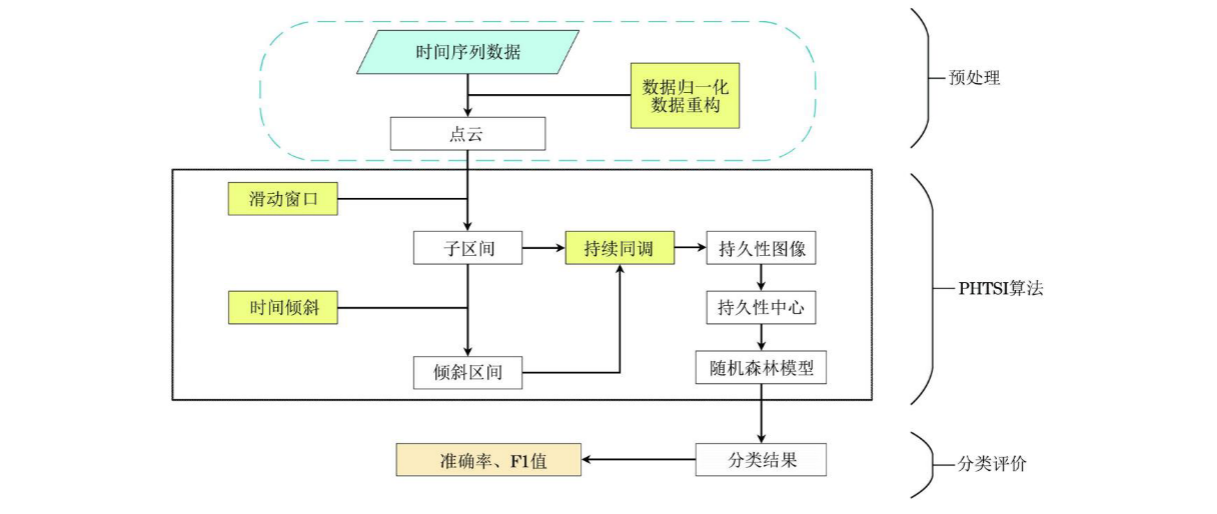
\includegraphics[width=1.0\textwidth]{figure/严银凯示意图.png}
    \caption{严银凯PHTSI算法示意图。}
\end{figure}

\subsubsection{特征化时间序列}
在标准的时间序列拓扑表示构建方法之外,为了更灵活地融入领域特定知识并优化持久同调的分析效果,Heo 与 Jung \cite{2} 近期提出了一种新颖的框架。该方法的核心在于引入了“特征化时间序列 (featured time series)”与“影响向量 (influence vector)”的概念,旨在通过调整时间序列的图表示来定制化持久同调的计算过程。

首先,一个特征化时间序列 $(\hat{T}, g)$ 由两部分构成:其一是特征增强的时间序列 $\hat{T}$,它将原始时间序列 $T$ 与一个特征组件 $T_f$ 配对,即 $\hat{T}(t) = (T(t), T_f(t))$。这里的特征组件 $T_f(t)$ 可以包含与单个时间点 $T(t)$ 相关的0阶特征(例如,某时刻的湿度状况)以及与相邻时间点对 $\{T(t_k), T(t_{k+1})\}$ 相关的1阶特征(例如,温度变化的幅度)。这些特征通常来源于特定领域的知识。其二是影响向量 $g$,它是一个非负实值函数,为每一个定义的特征(以及无特征状态)赋予一个“影响值”,用以量化该特征在后续分析中的重要性 。

该方法接着利用特征化时间序列 $(\hat{T}, g)$ 来构建一个加权图 $G=(V,E,\hat{W}_V,\hat{W}_E)$。其中,顶点集 $V$ 由时间序列中的观测值构成,边集 $E$ 通常连接连续的观测值。关键在于顶点权重函数 $\hat{W}_V$ 和边权重函数 $\hat{W}_E$ 的计算。它们并非简单地基于原始序列的频率,而是通过结合特征的出现次数和影响向量 $g$ 来确定。具体地,设 $F^0 = \{r_1, ..., r_m\}$ 为0阶特征集,$F^1 = \{s_1, ..., s_l\}$ 为1阶特征集。定义0阶计数矩阵 $C_0=(c_{ij}^0)$,其中 $c_{ij}^0$ 表示顶点 $v_i$ 与特征 $r_j$ (或无0阶特征状态 $\emptyset^0$) 在 $\hat{T}$ 中共同出现的次数。类似地,定义1阶计数矩阵 $C_1=(c_{ij}^1)$,其中 $c_{ij}^1$ 表示边 $e_i$ 与特征 $s_j$ (或无1阶特征状态 $\emptyset^1$) 在 $\hat{T}$ 中共同出现的次数。若影响向量 $g$ 对应0阶和1阶特征的分量分别为 $\vec{g_0} = (g(\emptyset^0), g(r_1), ..., g(r_m))$ 和 $\vec{g_1} = (g(\emptyset^1), g(s_1), ..., g(s_l))$,则顶点 $v_i$ 的权重和边 $e_i$ 的权重(也称为加权频率 $\hat{f}_{e_i}$)可以计算为:
\begin{equation}
\label{eq:featured_vertex_weight_revised}
\hat{W}_V(v_i) = (C_0 \cdot \vec{g_0})_i
\end{equation}
\begin{equation}
\label{eq:featured_edge_weight_revised}
\hat{W}_E(e_i) = \hat{f}_{e_i} = (C_1 \cdot (\vec{g_1} + \vec{1}))_i
\end{equation}
其中 $\vec{1}$ 是全1向量,用于确保在 $\vec{g_1}=\vec{0}$ 时边权重与传统频率定义一致 。

随后,基于这个加权的图 $\hat{G}^g$,定义了节点间的距离度量 $\hat{d}$。对于图中的一条边 $e=\{a,b\}$,其长度 $L^g(e)$ 不仅考虑了其加权频率的倒数 $(\hat{W}_E(e))^{-1}$,还通过一个激活函数 $\rho$ (如 $\rho(z)=1-e^{-z^2}$ 对于 $z \ge 0$) 引入了与该边连接的两个顶点 $a,b$ 的加权频率 $\hat{W}_V(a)$ 和 $\hat{W}_V(b)$ 的影响:
\begin{equation}
\label{eq:featured_edge_length_revised}
L^g(e) = (\hat{W}_E(e))^{-1} - \alpha (\rho(\hat{W}_V(a) + \hat{W}_V(b)))
\end{equation}
其中 $\alpha = \min_{e' \in E} (\hat{W}_E(e'))^{-1}$ 是一个归一化因子,确保边长非负。两个顶点 $v,w$ 之间的距离 $\hat{d}(v,w)$ 则定义为连接它们的最短路径上所有边长度 $L^g(e)$ 之和 。
\begin{equation}
\label{eq:featured_distance_revised}
\hat{d}(v,w) = \min_{p: v \leadsto w} \left\{ \sum_{e \in p} L^g(e) \right\}
\end{equation}
这个经过特征和影响向量调整的距离度量 $(V, \hat{d})$ 构成了计算持久同调(例如通过Vietoris-Rips滤过)的基础。通过改变影响向量 $g$,研究者可以探索不同领域知识对时间序列拓扑结构的影响。Heo 与 Jung 证明了这种方法的一个重要性质:持久性图对于影响向量 $g$ 的变化是稳定的,即满足 $D_B(\text{dgm}_p(g), \text{dgm}_p(g')) \le C ||g-g'||_\infty$,其中 $D_B$ 是瓶颈距离,$C$ 是一个常数。这种稳定性保证了该增强方法在调整领域知识影响时的鲁棒性和结果的可靠性。
\begin{table}[htbp]
    \centering
    \caption{传统点云嵌入与Heo \& Jung特征化时间序列方法的简明对比}
    \label{tab:embedding_comparison_concise}
    \begin{tabular}{>{\raggedright\arraybackslash}p{0.25\textwidth} >{\raggedright\arraybackslash}p{0.35\textwidth} >{\raggedright\arraybackslash}p{0.35\textwidth}}
    \toprule
    \textbf{比较维度} & \textbf{传统点云嵌入 (以TDE为例)} & \textbf{Heo \& Jung 的特征化方法} \\
    \midrule
    核心目标/输出 &
    在欧几里得空间($\mathbb{R}^m$)中重构几何点云,代表系统状态。 &
    构建一个赋权图,并基于此定义一个可调整的度量空间 $(V, \hat{d})$ 作为拓扑分析输入。 \\
    \addlinespace
    距离度量来源 &
    通常是嵌入点之间的欧几里得距离。 &
    基于图的边/点权重(由特征和影响向量决定)定义的最短路径距离 $\hat{d}(v,w)$。 \\
    \addlinespace
    领域知识整合 &
    通常不直接在构造中融入,主要通过参数选择间接体现。 &
    通过“特征化时间序列”和“影响向量”显式、量化地融入距离度量的计算中。 \\
    \addlinespace
    调整机制 &
    主要调整嵌入维度 $d$ 和时间延迟 $\tau$。 &
    主要调整“影响向量” $g$,改变特征对距离度量的影响。 \\
    \addlinespace
    “增强”体现 &
    优化参数以期更好地“展开”吸引子。 &
    通过影响向量主动“调制”点间距离,使度量空间更能反映关注的结构。 \\
    \addlinespace
    理论稳定性 &
    依赖Takens等定理(理想条件);对参数选择敏感。 &
    Heo \& Jung 证明了持久性图对影响向量变化具有稳定性,增强了调整时的可靠性。 \\
    \bottomrule
    \end{tabular}
    \end{table}
\subsection{从点云构建复形过滤}
将时间序列数据转换为高维欧几里得空间 $\mathbb{R}^d$ 中的点云 $P$ 是进行拓扑数据分析的前置步骤。然而,点云本身仅为离散点的集合,缺乏描述点与点之间连接关系或更高维度结构(如环、空腔)的内在信息。拓扑数据分析,特别是持续同调(Persistent Homology, PH),正是通过分析点云数据所隐含的这种高阶结构来量化数据的“形状”特征。至关重要的是,持续同调并非直接作用于原始点云,而是作用于从点云数据构建的单纯复形(Simplicial Complex)或类似组合结构(如立方复形)之上。更进一步,持续同调的核心在于研究拓扑特征如何在不同尺度(scale)下演化并持续存在。因此,仅仅构建单个复形是不够的,必须构建一个随尺度参数变化的复形序列,即所谓的过滤(Filtration)。这一过程是连接点云的几何表示与持续同调所揭示的拓扑不变量之间的关键桥梁。

从点云 $P \subset \mathbb{R}^d$ 构建单纯复形的基本思想是基于点的“邻近性”:若一组点在某种意义上彼此足够接近,则它们应共同构成一个结构单元(即单形)。这种邻近度通常由一个非负的尺度参数 $\epsilon$ 来量化。随着 $\epsilon$ 的增加,越来越多的点集被认为是“邻近”的,从而允许形成更高维度的单形,使得复形的整体结构逐渐丰富和复杂化。这种随 $\epsilon$ 增长而形成的、在集合包含关系上单调递增的复形序列 $K_{\epsilon_0} \subset K_{\epsilon_1} \subset \dots \subset K_{\epsilon_n}$(其中 $0 \le \epsilon_0 < \epsilon_1 < \dots < \epsilon_n$)即构成了过滤流,这是计算持续同调的标准输入。

\subsubsection{Vietoris-Rips复形}
在信号分析的拓扑方法中,一个核心步骤是从时间序列数据生成点云,并进一步构造单纯复形以揭示其潜在的几何与拓扑特性。这里关注Perea等人\cite{perea2015sliding}运用的滑动窗口嵌入(Sliding Window Embedding)技术以及由此产生的点云所构建的Rips复形。

首先,介绍滑动窗口嵌入方法。假设有一个在实数区间上定义的函数 $f$(例如,一个时间序列信号)。选择一个正整数 $M$ 和一个正实数 $\tau$(时间延迟)。在时间点 $t \in \mathbb{R}$,函数 $f$ 到 $\mathbb{R}^{M+1}$ 维空间的滑动窗口嵌入点 $SW_{M,\tau}f(t)$ 定义为:
\begin{equation}
SW_{M,\tau}f(t) = \begin{bmatrix} f(t) \\ f(t+\tau) \\ \vdots \\ f(t+M\tau) \end{bmatrix}
\end{equation}
通过在不同的时间点 $t$ 上进行采样,可以得到一个点云集合,即滑动窗口点云(Sliding Window Point Cloud)。这个点云是后续拓扑分析的基础。此嵌入的一个关键参数是窗口大小(window-size)$M\tau$。

获得了滑动窗口点云 $X$(通常是一个紧致集,例如由有限个采样点构成)后,采用Rips复形进行构造。给定一个距离参数 $r \ge 0$,点云 $X$ 上的Rips复形,记作 $R_r(X)$,是一个单纯复形,其顶点集即为点云 $X$ 中的点。一个包含 $k+1$ 个顶点 $\{x_0, x_1, \ldots, x_k\}$ 的集合构成 $R_r(X)$ 中的一个 $k$-单纯形(记作 $[x_0, x_1, \ldots, x_k]$),当且仅当该集合中任意两个不同顶点 $x_i, x_j$ 之间的欧氏距离(或其他定义好的度量)满足以下条件:
\begin{equation}
\|x_i - x_j\| \leq r \quad \forall 0 \leq i < j \leq k
\end{equation}
值得注意的是,Rips复形的构造仅依赖于其一维骨架(即边):一个高维单纯形被包含在复形中,当且仅当它的所有边(即所有顶点对)都满足上述距离条件。通过改变参数 $r$ 的值,可以得到一个嵌套的复形序列 $R_0(X) \subset R_{r_1}(X) \subset \ldots \subset R_{r_m}(X)$,这构成了Rips过滤(Rips filtration),是计算持久同调的基础。

这种从信号到点云再到过滤复形的过程,使得可以运用持久同调来量化信号的周期性等特征。

%插入图片
\begin{figure}[thbp!]
    \centering
    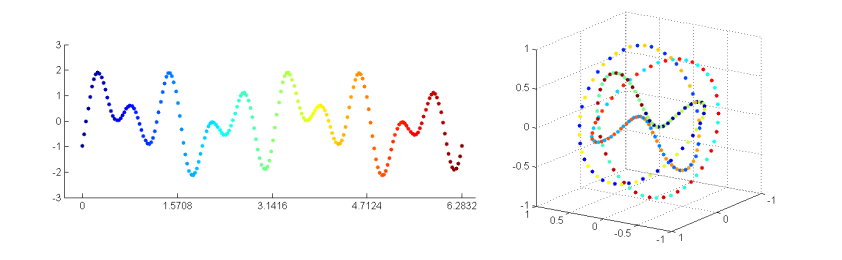
\includegraphics[width=0.8\textwidth]{figure/滑动窗口嵌入示意图、.png}
    \caption{滑动窗口嵌入点云示意图}
\end{figure}

\begin{table}[htbp]
    \centering
    \caption{不同算法在合成数据集上的分类性能 (AUC 值)}
    \label{tab:auc_results}
    \begin{tabular}{@{}llcccc@{}}
    \toprule
    \multirow{2}{*}{信号类型} & \multirow{2}{*}{噪声水平 (SD)} & \multicolumn{4}{c}{算法的AUC值} \\
    \cmidrule(l){3-6}
     &  & JTK & LS & PH & SW1P \\
    \midrule
    \multirow{3}{*}{Cosine (余弦波)} & 0  & 1.00 & 1.00 & 1.00 & 1.00 \\
                                   & 25 & 1.00 & 1.00 & 0.97 & 1.00 \\
                                   & 50 & 0.96 & 0.99 & 0.78 & 0.98 \\
    \midrule
    \multirow{3}{*}{Damped (阻尼波)} & 0  & 1.00 & 1.00 & 1.00 & 1.00 \\
                                   & 25 & 0.94 & 0.98 & 0.65 & 0.90 \\
                                   & 50 & 0.56 & 0.66 & 0.59 & 0.71 \\
    \midrule
    \multirow{3}{*}{Peaked (尖峰波)} & 0  & 1.00 & 1.00 & 1.00 & 1.00 \\
                                   & 25 & 0.99 & 1.00 & 0.92 & 0.99 \\
                                   & 50 & 0.72 & 0.86 & 0.77 & 0.87 \\
    \midrule
    \multirow{3}{*}{Trended (趋势波)} & 0  & 1.00 & 1.00 & 1.00 & 1.00 \\
                                    & 25 & 1.00 & 1.00 & 0.98 & 0.99 \\
                                    & 50 & 0.93 & 0.97 & 0.81 & 0.93 \\
    \bottomrule
    \end{tabular}
    \footnotesize
    \newline
    \textit{注:数据来源于 Perea 和 Harer 的论文中图6所示的ROC曲线分析。SW1P是该论文提出的方法。LS代表Lomb-Scargle,PH代表通用的持续同调方法)。}
    \end{table}


\subsubsection{witness复形}
当点云 $P$ 的规模非常大时,构建VR复形的计算开销会非常高。为了解决这个问题,可以使用 Witness 复形\cite{de2004topological}。Witness 复形是在点云 $P$ 的一个(通常较小的)子集 $Q = \{q_1, q_2, \ldots, q_M\} \subset P$ (称为地标点,landmark points) 上构建的,但其结构依然受到整个点云 $P$ (称为 witness 点) 的影响。地标点可以通过最大最小采样 (maxmin) 或随机采样等方法从 $P$ 中选取。Mittal\cite{mittal2017topological}论文中提到了两种类型的Witness复形,其定义基于“被见证”的概念:

一个由地标点构成的单纯形 $\sigma = [q_{j_0}, q_{j_1}, \ldots, q_{j_k}]$ (其中 $q_{j_l} \in Q$) 被点云 $P$ 中的一个点 $x \in P$ (称为 witness) 所“弱见证”(weakly witnessed),若对于 $\sigma$ 中的每一个顶点 $q \in \{q_{j_0}, \ldots, q_{j_k}\}$ 以及任意一个不在 $\sigma$ 中的地标点 $p \in Q \setminus \{q_{j_0}, \ldots, q_{j_k}\}$,都满足以下距离关系:
\begin{equation}
d(q, x) \le d(p, x)
\end{equation}
这个条件意味着,相对于 witness 点 $x$ 而言,单纯形 $\sigma$ 中的所有顶点 $q$ 比任何不在 $\sigma$ 中的地标点 $p$ 都更近(或等近)。

基于此,弱 Witness 复形 $\mathcal{W}_{weak}(P, Q)$ 定义为包含所有那些能够被点云 $P$ 中至少一个点 $x \in P$ 所弱见证的地标单纯形 $\sigma \subseteq Q$ 的集合。

进一步地,强 Witness 复形 $\mathcal{W}_{strong}(P, Q)$ 对见证条件有更严格的要求。一个地标单纯形 $\sigma = [q_{j_0}, \ldots, q_{j_k}]$ 属于强 Witness 复形,如果它被某个 $x \in P$ 所弱见证,并且对于这个 $x$,它到 $\sigma$ 的所有顶点的距离都相等:
\begin{equation}
d(q_{j_0}, x) = d(q_{j_1}, x) = \ldots = d(q_{j_k}, x)
\end{equation}
这两种Witness复形的构造都依赖于地标点和原始点云中 witness 点之间的距离关系,从而在降低计算复杂度的同时,试图捕捉原始点云的拓扑特征。

通过改变VR复形的尺度参数 $\epsilon$ 或Witness复形的选取方式(例如,地标点的数量或特定的见证半径,尽管本论文的定义更侧重相对距离),可以构建一个过滤的单纯复形序列,这是进行持久同调分析的基础。
